\subsection{Identifying Theories via Implicit Isomorphisms}\label{sec:inverse}

In this section, we introduce several language extensions that introduce implicit isomorphisms.

Note that because identity morphisms are implicit, our uniqueness requirement for implicit morphisms implies that two theories $S$ and $T$ must be isomorphic if there are implicit morphisms in both directions.
Moreover, making a pair of isomorphisms implicit is well-formed if there are no other implicit morphisms between $S$ and $T$ yet.

\paragraph{Renamings}
We say that a named morphism $r:S\to T=\{\ldots\}$ is a \textbf{renaming} if
\begin{compactitem}
 \item all assignments in its body are of the form $c:=c'$ for $T$-constants $c'$ without definiens
 \item every such $T$-constants $c'$ occurs in exactly one assignment.
\end{compactitem}
Clearly, every renaming is an isomorphism.
The inverse morphisms contains the flipped assignments $c':=c$.

We make the following extension to syntax and semantics:
\begin{compactitem}
  \item A morphism declaration $r:s\to t=\{\ldots\}$ may carry the attribute \keyword{renaming}.
  \item This is well-formed if there are no implicit morphism between $s$ and $t$ yet.
  \item In that case, we define $r\in\IMo{s}{t}$ and $r^{-1}\in\Mo{t}{s}$.
\end{compactitem}

\begin{example}
	Consider a variation of the theory $\cn{Monoid}$ from \autoref{syn:incl} in a different library:
	\begin{mmtcode}
Monoid2 =
  M: type
  connective : M ⟶ M ⟶ M	 # 1 ∘ 2 
  neutral	: M
\end{mmtcode}
This theory is isomorphic to the previously introduced theory $\cn{Monoid}$ under the trivial renaming
	\begin{mmtcode}
Monoids : Monoid2 -> Monoid =
  M 		:= U
  connective 	:= op 
  neutral	:= unit
\end{mmtcode}
\end{example}

\paragraph{Definitional Extensions}
We say that the named theory $t$ is a \textbf{definitional extension} of $S$ if $t=S$ or the body of $t$ contains
\begin{compactitem}
 \item only constant declarations with definiens,
 \item only include declarations of theories that are definitional extensions of $S$.
\end{compactitem}
\begin{example}
	Imagine extending the theory $\cn{Group}$ from \autoref{syn:incl} by provable theorems:
		\begin{mmtcode}
Group_Theorems =
  include Group
  inverse_idem : ⊦∀[x] (x⁻¹)⁻¹≐x 	= (proof)
\end{mmtcode}
\end{example}

If $t$ is a definitional extension of $S$, it is easy to prove that $t$ and $S$ are isomorphic: both isomorphisms map all constants without definiens to themselves. In particular, the isomorphism $S\to t$ maps $S$-constants to themselves and expands the definiens of all other constants.

We make the following extension to syntax and semantics:
\begin{compactitem}
  \item An include declaration $\icl{s}$ of a named theory $s$ inside theory $t$ may carry the attribute \keyword{definitional}.
  \item In that case, we define $\id{s}\in\IMo{t}{s}$ (in addition to the implicit morphism $\id{t}\in\IMo{s}{t}$ which is induced by the inclusion).
\end{compactitem}
\begin{example}
	We adapt our theory $\cn{Group\_Theorems}$ with the newly introduced keyword, which allows us to extend $\cn{Group}$ directly while having the new theorem $\cn{inverse\_idem}$ available:
		\begin{mmtcode}
Group_Theorems =
  definitional include Group
  inverse_idem : ⊦∀[x] (x⁻¹)⁻¹≐x 	= (proof)

More_Theorems =
  include ?Group
  some_other_theorem : ⊦ ??	= (proof using inverse_idem)
\end{mmtcode}
\end{example}

\begin{remark}[Conservative Extensions]
A definitional extension is a special case of a conservative extension.
More generally, all retractable extensions are conservative, i.e., all extensions $S\harr T$ such that there is a morphism $r:T\to S$ such that $r$ is the identity on $S$.

But we cannot make the retractions implicit morphisms in general because they are not necessarily isomorphisms.
\end{remark}

\paragraph{Canonical Isomorphisms}
If we have isomorphisms $m:s\to t$ and $n:t\to s$, we simply spell them out in morphism declarations and add the keyword \keyword{implicit} to both.
This requires no language extensions.

\begin{example}\label{group:iso}
Having declared the morphism $\cn{DG2G}$ (as in \autoref{ex:dg2g}) implicit, we do the same with the reverse morphism  $\cn{G2DG}$:
\begin{mmtcode}
implicit G2DG : Group -> DivisionGroup =
  U := U
  op := [a,b] a / ((unit/unit) / b) 
  unit := unit/unit
  inverse := [a] (unit/unit) / a
\end{mmtcode}
\end{example}

While the first one of these isomorphism declarations is straightforward, the second one requires checking that $m$ and $n$ are actually isomorphisms.
Otherwise, the uniqueness condition would be violated.
Thus, we have to check $m;n=\id{s}$ and $n;m=\id{t}$.
In general, the equality of two morphisms $f,g:A\to B$ is equivalent to $\vdash_B f(c)=g(c)$ for all $c:E\in\flt{A}$.
Thus, if equality of expressions is decidable in the logic that \mmt is instantiated with, then \mmt can check this directly.

However, this does not work in practice.
Already elementary examples require stronger, undecidable equality relations are used:

\begin{example}
Consider the isomorphism from Ex.~\ref{group:iso}.
The result of mapping $x\circ y$ from $\cn{Group}$ to $\cn{DivGroup}$ and back is $x\circ(unit\circ y^{-1})^{-1}$.
Clearly, the group axioms imply that this is equal to $x\circ y$.
But formally that requires working with the undecidable equality of first-order logic.
\end{example}

Therefore, in our running example, we only make one of the two isomorphisms implicit.

In the sequel, we design a general solution to this problem.
It allows systematically proving the equality of two morphisms and using that to make both isomorphisms implicit.
This is novel work, but it requires significant prerequisites and is only peripherally related to implicit morphisms.
Therefore, we only sketch the idea and leave the details to future work.

We add a language feature to \mmt to prove equalities between morphisms:
We add the productions
\begin{grammar}
Dia   & \rep{(TDec \alt MDec\alt MEq)}  &\\
MEq   & \keyword{equal} M=M:T\to T by \{\rep{Ass}\} &\\
\end{grammar}

%Firstly, the intuition of $\keyword{equality} T = \{c:=E,\ldots\}$ is that it provides to every base type $c:\type$ of $T$ a judgment $E:c\to c\to \type$ that defines the $T$-specific equality relation for objects of type $c$.
%Technically, this must be a binary logical relation in the sense of \cite{RS:logrels:12} on $\id{T}$.
%As described in \cite{RS:logrels:12}, this induces an equality predicate $\cn{Equal}_E:E\to E\to \type$ on every type $E$.

We define the declaration $M=N:S\to T by \{\sigma\}$ to be well-formed iff
\begin{compactitem} 
  \item $M:S\to T$ and $N:S\to T$ are well-formed morphisms
  \item $\sigma$ contains exactly one assignment $c:=p$ for every $(c:E)\in\flt{S}$
  \item for each of these assignments $c:=p$, the term $p$ is a proof of $\vdash_T M(c)=N(c)$.
\end{compactitem}

To make $m$ and $n$ from above implicit isomorphisms, we have to do three things: define $m$ and $n$, prove the equalities of $m;n=\id{s}$ and $n;m=\id{t}$, and make $m$ and $n$ implicit.
Note that we cannot make both $m$ and $n$ implicit right away because that is only well-formed after proving the equalities.)
Thus, we define a new attribute \keyword{implicit-later}, which states that a morphism should be considered implicit as soon as subsequent equality proves make it well-formed to do so.

\begin{example}[Isomorphisms]
We can now add declarations
 \[\keyword{implicit}:\cn{DG2G}:\cn{DivGroup}\to\cn{Group}=\text{(as above)}\]
 \[\keyword{implicit-later}:\cn{G2DG}:\cn{Group}\to\cn{DivGroup}=\text{(as above)}\]
 \[\keyword{equal}\cn{G2DG};\cn{DG2G}=\id{\cn{Group}}:\cn{Group}\to\cn{Group}=\text{(omitted)}\]
 \[\keyword{equal}\cn{DG2D};\cn{G2DG}=\id{\cn{DivGroup}}:\cn{DivGroup}\to\cn{DivGroup}=\text{(omitted)}\]
where the isomorphisms are as above and we omit all the equality proofs.
\end{example}

\subsection{Fine-Granular and Flexible Theory Hierarchies}
A common problem when defining modular theory hierarchies is that the most natural include-hierarchy for the most important theories is not necessarily the same as the most comprehensive hierarchy.
For example, Ex.~\ref{syn:incl} defines \cn{Group} with an include from \cn{Monoid}.
Instead, we could include \cn{Monoid} into the intermediate theory \cn{CancellationMonoid} and include that into \cn{Group}.
This change is not possible in retrospect --- changing the theory hierarchy (which is one of the most fundamental structures of a library) usually presents an insurmountable refactoring problem.
So instead we could systematically build a hierarchy that uses every intermediate theory (as done in \cite{mathscheme}).
But this yields a very deep and complex hierarchy that is hard to navigate for casual users.
Moreover, it does not protect us from later on discovering yet another intermediate theory that should have been added.

Implicit morphisms provide a simple solution to this problem because they behave effectively like inclusions but can be added later on.
In the above example, we would
\begin{compactitem}
 \item define \cn{CancellationMonoid} with an include from \cn{Monoid},
 \item keep \cn{Group} as it is, i.e., also with an include \cn{Monoid},
 \item add an implicit morphism $\cn{CancellationMonoid}\to\cn{Group}$.
\end{compactitem}
\medskip

As a more complex example, we have built a hierarchy of theories between \cn{Band} and \cn{Semilattice}.
\ednote{@DM: this is not quite the lattice from the Wikipedia page: it consists of the 3x3 square plus Bands at the top}
All of these theories are of the form $t=\{\icl{\cn{Band}},\,a:\vdash F\}$, where $F$ is a universally quantified equational axiom.\footnote{All varieties of bands can be axiomatized in this way.}
In particular, $\cn{SemiLattice}=\{\icl{\cn{Band}},\,a:\vdash \forall [x]\forall [y] x\circ y\doteq y\circ x\}$.
Fig.~\ref{fig:bands} shows these theories.

There are various morphisms between them that describe the lattice structure of the corresponding varieties of bands.
All of these map the constants from \cn{Band} to themselves and the axiom $a$ to a proof.%
\footnote{Our formalization of the lattice of bands using implicit morphisms can be found at \url{https://gl.mathhub.info/MitM/smglom/blob/devel/source/algebra/bands.mmt}.}
We make all of these morphisms implicit.
It is straightforward to prove that the diagram commutes: any two morphisms are identical except for assignment for the axiom.
Here, \mmt can discharge the proof obligation easily using proof irrelevance.

\begin{figure}\begin{center}
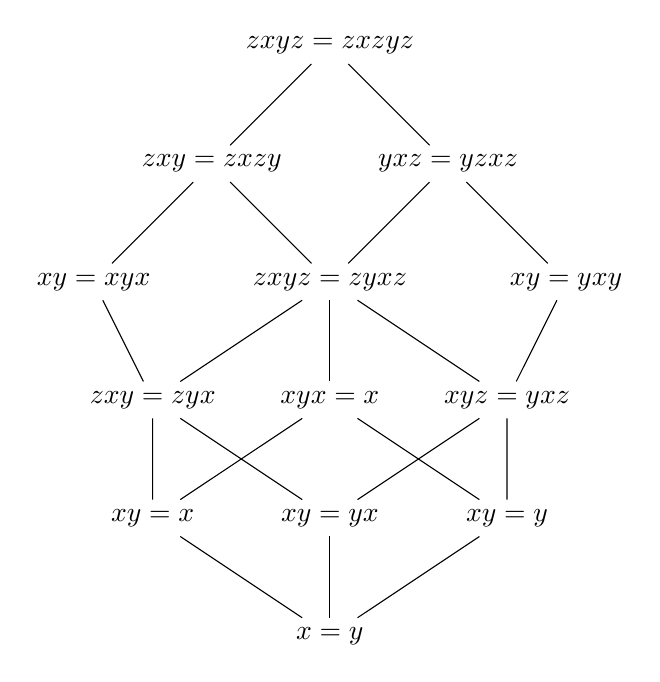
\begin{tikzpicture}[scale=1.5]
  \node (s1) at (0,0) {$zxyz=zxzyz$};
  
  \node (s2a) at (-1,-1) {$zxy=zxzy$};
  \node (s2b) at (1,-1) {$yxz=yzxz$};
  \draw (s1) to (s2a) {};
  \draw (s1) to (s2b) {};
  
  \node (s3a) at (-2,-2) {$xy=xyx$};
  \node (s3b) at (0,-2) {$zxyz=zyxz$};
  \node (s3c) at (2,-2) {$xy=yxy$};
  \draw (s2a) to (s3a) {};
  \draw (s2a) to (s3b) {};
  \draw (s2b) to (s3b) {};
  \draw (s2b) to (s3c) {};
  
  \node (s4a) at (-1.5,-3) {$zxy=zyx$};
  \node (s4b) at (0,-3) {$xyx=x$};
  \node (s4c) at (1.5,-3) {$xyz=yxz$};
  \draw (s3a) to (s4a) {};
  \draw (s3b) to (s4a) {};
  \draw (s3b) to (s4b) {};
  \draw (s3b) to (s4c) {};
  \draw (s3c) to (s4c) {};
  
  
  \node (s5a) at (-1.5,-4) {$xy=x$};
  \node (s5b) at (0,-4) {$xy=yx$};
  \node (s5c) at (1.5,-4) {$xy=y$};
  \draw (s4a) to (s5a) {};
  \draw (s4a) to (s5b) {};
  \draw (s4b) to (s5a) {};
  \draw (s4b) to (s5c) {};
  \draw (s4c) to (s5b) {};
  \draw (s4c) to (s5c) {};
  
  \node (s6) at (0,-5) {$x=y$};
  \draw (s5a) to (s6) {};
  \draw (s5b) to (s6) {};
  \draw (s5c) to (s6) {};
  
  %\node[thy,inner sep=.3cm,fill=gray] (t1) at (0,0) {};
  %\node at (t1.north west) {$S$};
  %\node at (t1) {$D$};
  %\node[thy,inner sep=.5cm,fill=lightgray] (s2) at (2,0) {};
  %\node[thy,inner sep=.3cm,fill=gray] (t2) at (2,0) {};
  %\node at (t2.north west) {$T$};
  %\node at (t2) {$C$};
  %\draw[view] (t1) to[out=10,in=170] node[above] {$\sigma$} (t2);
\end{tikzpicture}

%
\includegraphics[width=0.6\textwidth]{bands}
\end{center}
\caption{The Lattice of Varieties of Bands}\label{fig:bands}
\end{figure}

%
%\begin{figure}
%\begin{tabular}{c|c}
%\begin{mmtcode}
%Band =
%  include ?SemiGroup
%  axiom_idemp : ⊦ ∀[x] x ∘ x ≐ x
%❚
%
%Regular =
%  include ?Band
%  axiom_regular : ⊦ ∀[x]∀[y]∀[z] 
%    z ∘ x ∘ z ∘ y ∘ z ≐ z ∘ x ∘ y ∘ z
%❚
%
%LeftNormal =
%  include ?Band
%  axiom_leftnormal : ⊦ ∀[x]∀[y]∀[z] 
%    z ∘ x ∘ z ∘ y ≐ z ∘ x ∘ y
%
%theory RightNormal =
%  include ?Band ❙
%  axiom_rightnormal : ⊦ ∀[x]∀[y]∀[z] 
%    y ∘ z ∘ x ∘ z ≐ y ∘ x ∘ z ❙ 
%❚
%
%theory Normal : ?Meta =
%  include ?Band ❙
%  axiom_normal :  ⊦ ∀[x]∀[y]∀[z] 
%    z ∘ x ∘ y ∘ z ≐ z ∘ y ∘ x ∘ z ❙
%❚
%\end{mmtcode} &
%\begin{mmtcode}
%implicit view Reg2LeftNormal : 
%    ?Regular -> ?LeftNormal =
%  include ?Band = ?Band ❙
%  axiom_regular = sketch "trivial" ❙
%❚
%
%implicit view Reg2RightNormal : 
%    ?Regular -> ?RightNormal =
%  include ?Band = ?Band ❙
%  axiom_regular = sketch "trivial" ❙
%❚
%
%implicit view LeftNormal2Normal : 
%    ?LeftNormal -> ?Normal =
%  include ?Band = ?Band ❙
%  axiom_leftnormal = sketch "trivial" ❙
%❚
%
%implicit view RightNormal2Normal : 
%    ?RightNormal -> ?Normal =
%  include ?Band = ?Band ❙
%  axiom_rightnormal = sketch "trivial" ❙
%❚
%\end{mmtcode}
%\end{tabular}
%
%\caption{Exemplary Theories for Some Varieties of Bands}\label{fig:bandsmmt}
%\end{figure}

\subsection{Transparent Refactoring}

A major drawback of using modular theories is that it can preclude transparent refactoring.
For example, consider a theory $t=\{\icl{r},\icl{s}\}$, and assume we want to move a constant declaration $D$ for the name $n$ from $r$ to $s$.
Thus, the change to should be straightforward as it does not change the semantics of $t$.

However, this is not a local change.
It also requires updating every qualified reference from $r?n$ to $s?n$.
Such references can occur anywhere where $t$ is used.
That may include theories that the person who does the refactoring does not know or does not have access to.
Even if the source files always use the unqualified reference $n$ (because the checker is smart enough to dynamically disambiguate them), this still requires a global rebuild to reach a consistent state again.

With implicit morphisms, we can solve this problem by making only the following local changes:
\begin{compactenum}
  \item We rename $s$ to $s'$.
  \item We delete the declaration $n:E$ from $s'$.
  \item We create new theories $r'=\{\icl{r},\,D\}$ and $s=\{\icl{s'},D\}$.
  \item We change $t$ to $t=\{\icl{r'},\icl{s'}\}$.
  \item We add an implicit morphism $s\to t$ that maps $s?n$ to $r'?n$.
\end{compactenum}
Now $t$ has the desired new structure.
But, all old references to $s?n$ stay well-formed so that no global changes are needed.

\ednote{@DM: maybe make a tikz for the before/after situations}